\documentclass{beamer}

\usepackage[utf8]{inputenc}
\usepackage{amssymb, amsmath}
\usepackage{ragged2e}
\usepackage{ulem}
\usepackage{listings}
\usepackage{amsthm}

\usepackage{graphicx}
\graphicspath{{./images/}}

\usetheme{metropolis}
\setbeamercolor{block title}{bg=red!20}

\usepackage{smartdiagram}
%%%%%%%%%%%%%%%%%%%%%%%%%%%%%%%%%%%%%%%%%%%%%%%%%%%%%%%%%%%%%%%
% Declaration for argmax
\DeclareMathOperator*{\argmax}{arg\,max}
\DeclareMathOperator*{\argmin}{arg\,min}

\title{English Word Suggestion Based on Part of Speech Ngram}
\subtitle{Hamana Laboratory, Gunma University}
\author{Borann Chanrathnak}

%%%%%%%%%%%%%%%%%%%%%%%%%%%%%%%%%%%%%%%%%%%%%%%%%%%%%%%%%%%%%%%
\begin{document}
\maketitle

%%%%%%%%%%%%%%%%%%%%%%%%%%%%%%%%%%%%%%%%%%%%%%%%%%%%%%%%%%%%%%%

\begin{frame}
\frametitle{Table of Contents}
\tableofcontents
\end{frame}

%%%%%%%%%%%%%%%%%%%%%%%%%%%%%%%%%%%%%%%%%%%%%%%%%%%%%%%%%%%%%%%
\section{Inspiration}
\begin{frame}{Inspiration}
    \begin{enumerate}
        \item Word suggestion on mobile devices
        \item Online digital writing tools
    \end{enumerate}
    \centering
    \visible<2->{
\includegraphics[width=3cm]{first}}
    \visible<3->{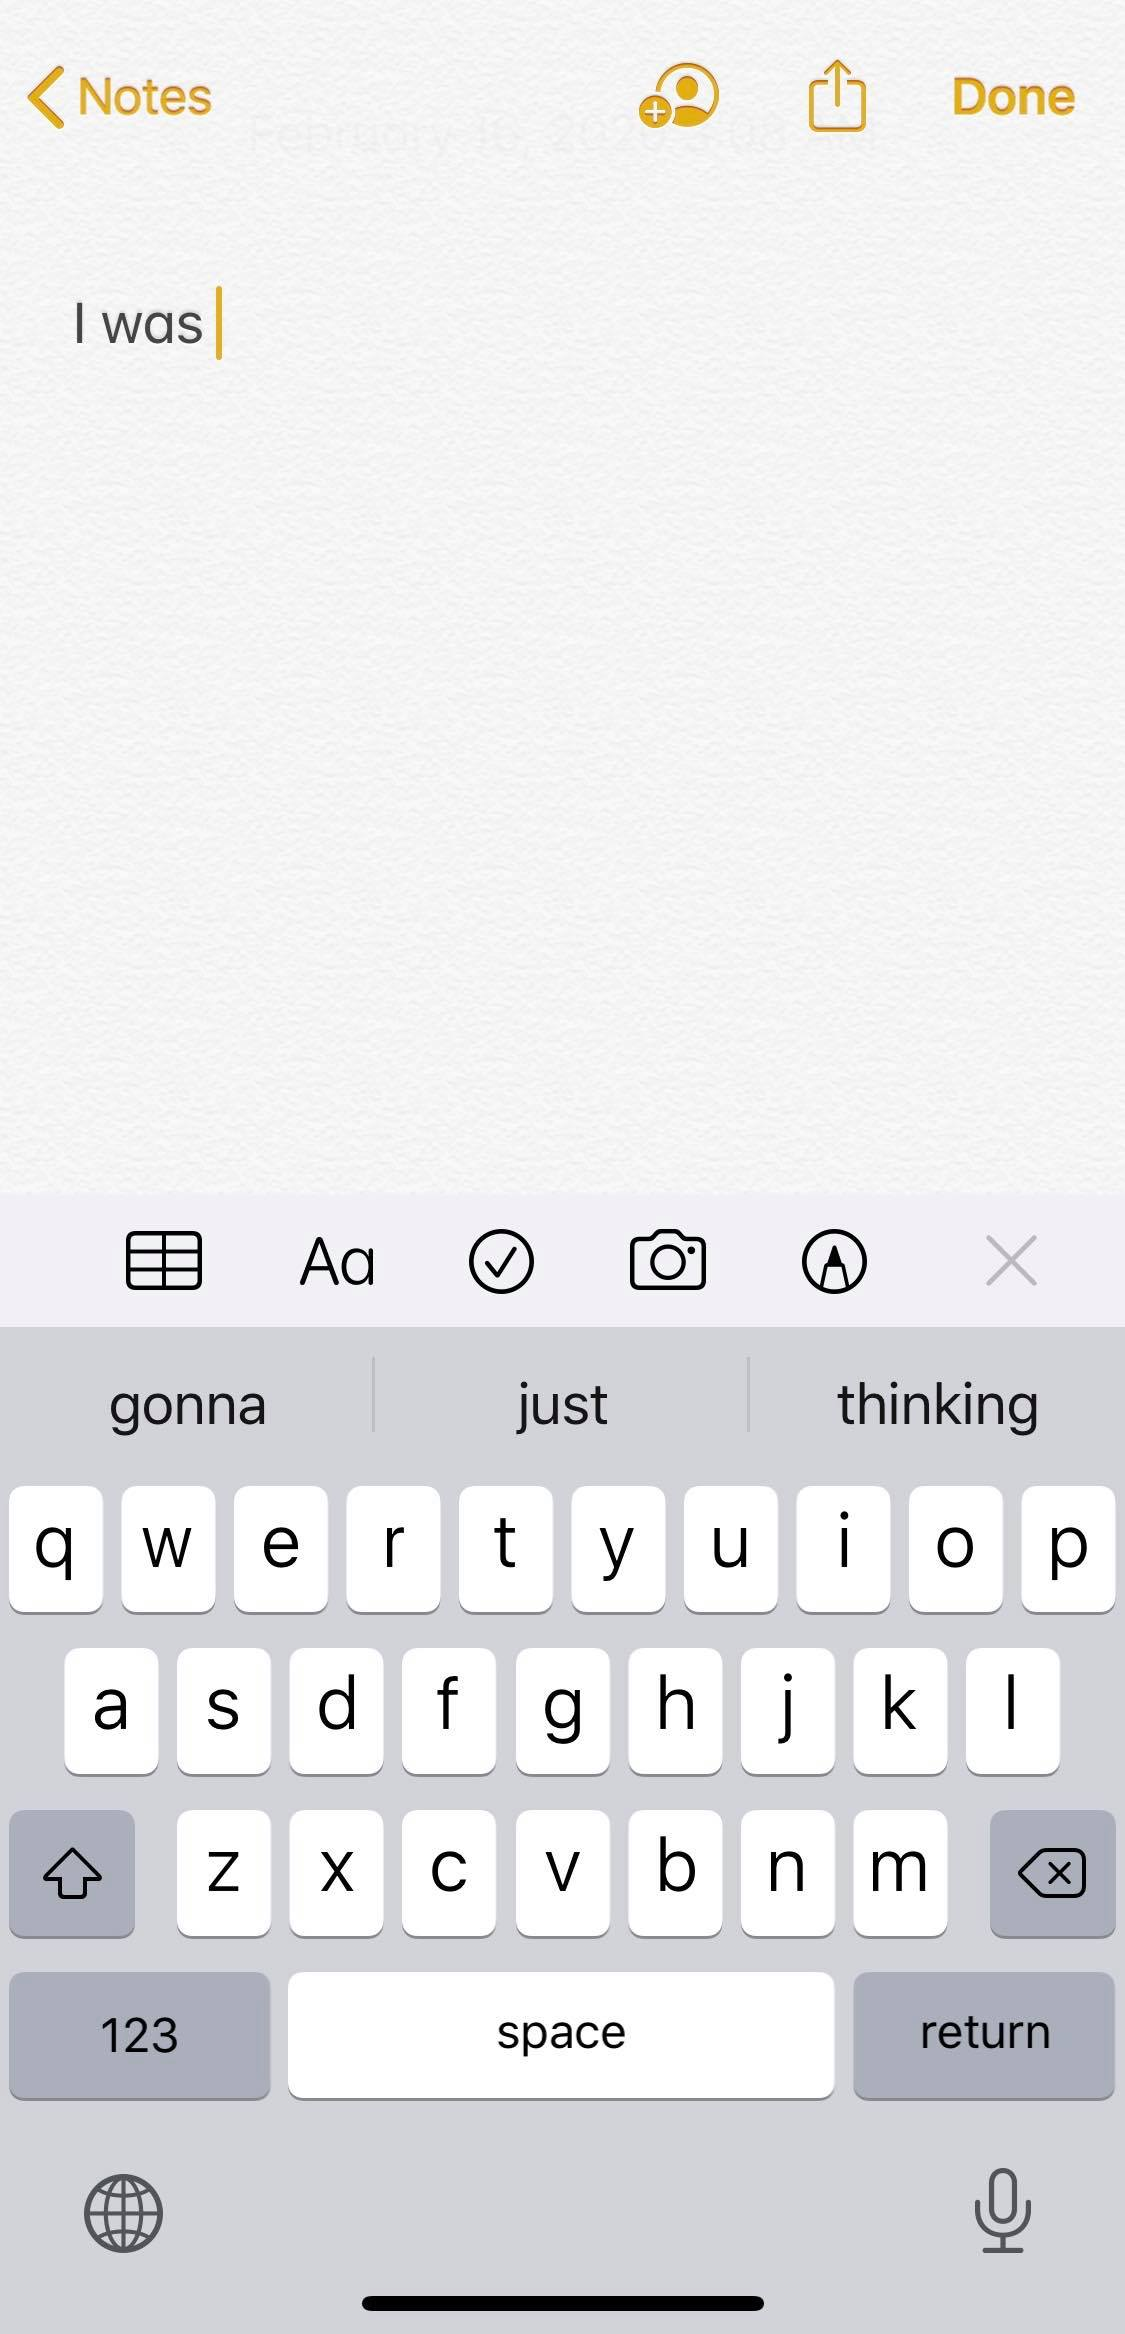
\includegraphics[width=3cm]{second}}
    \visible<4->{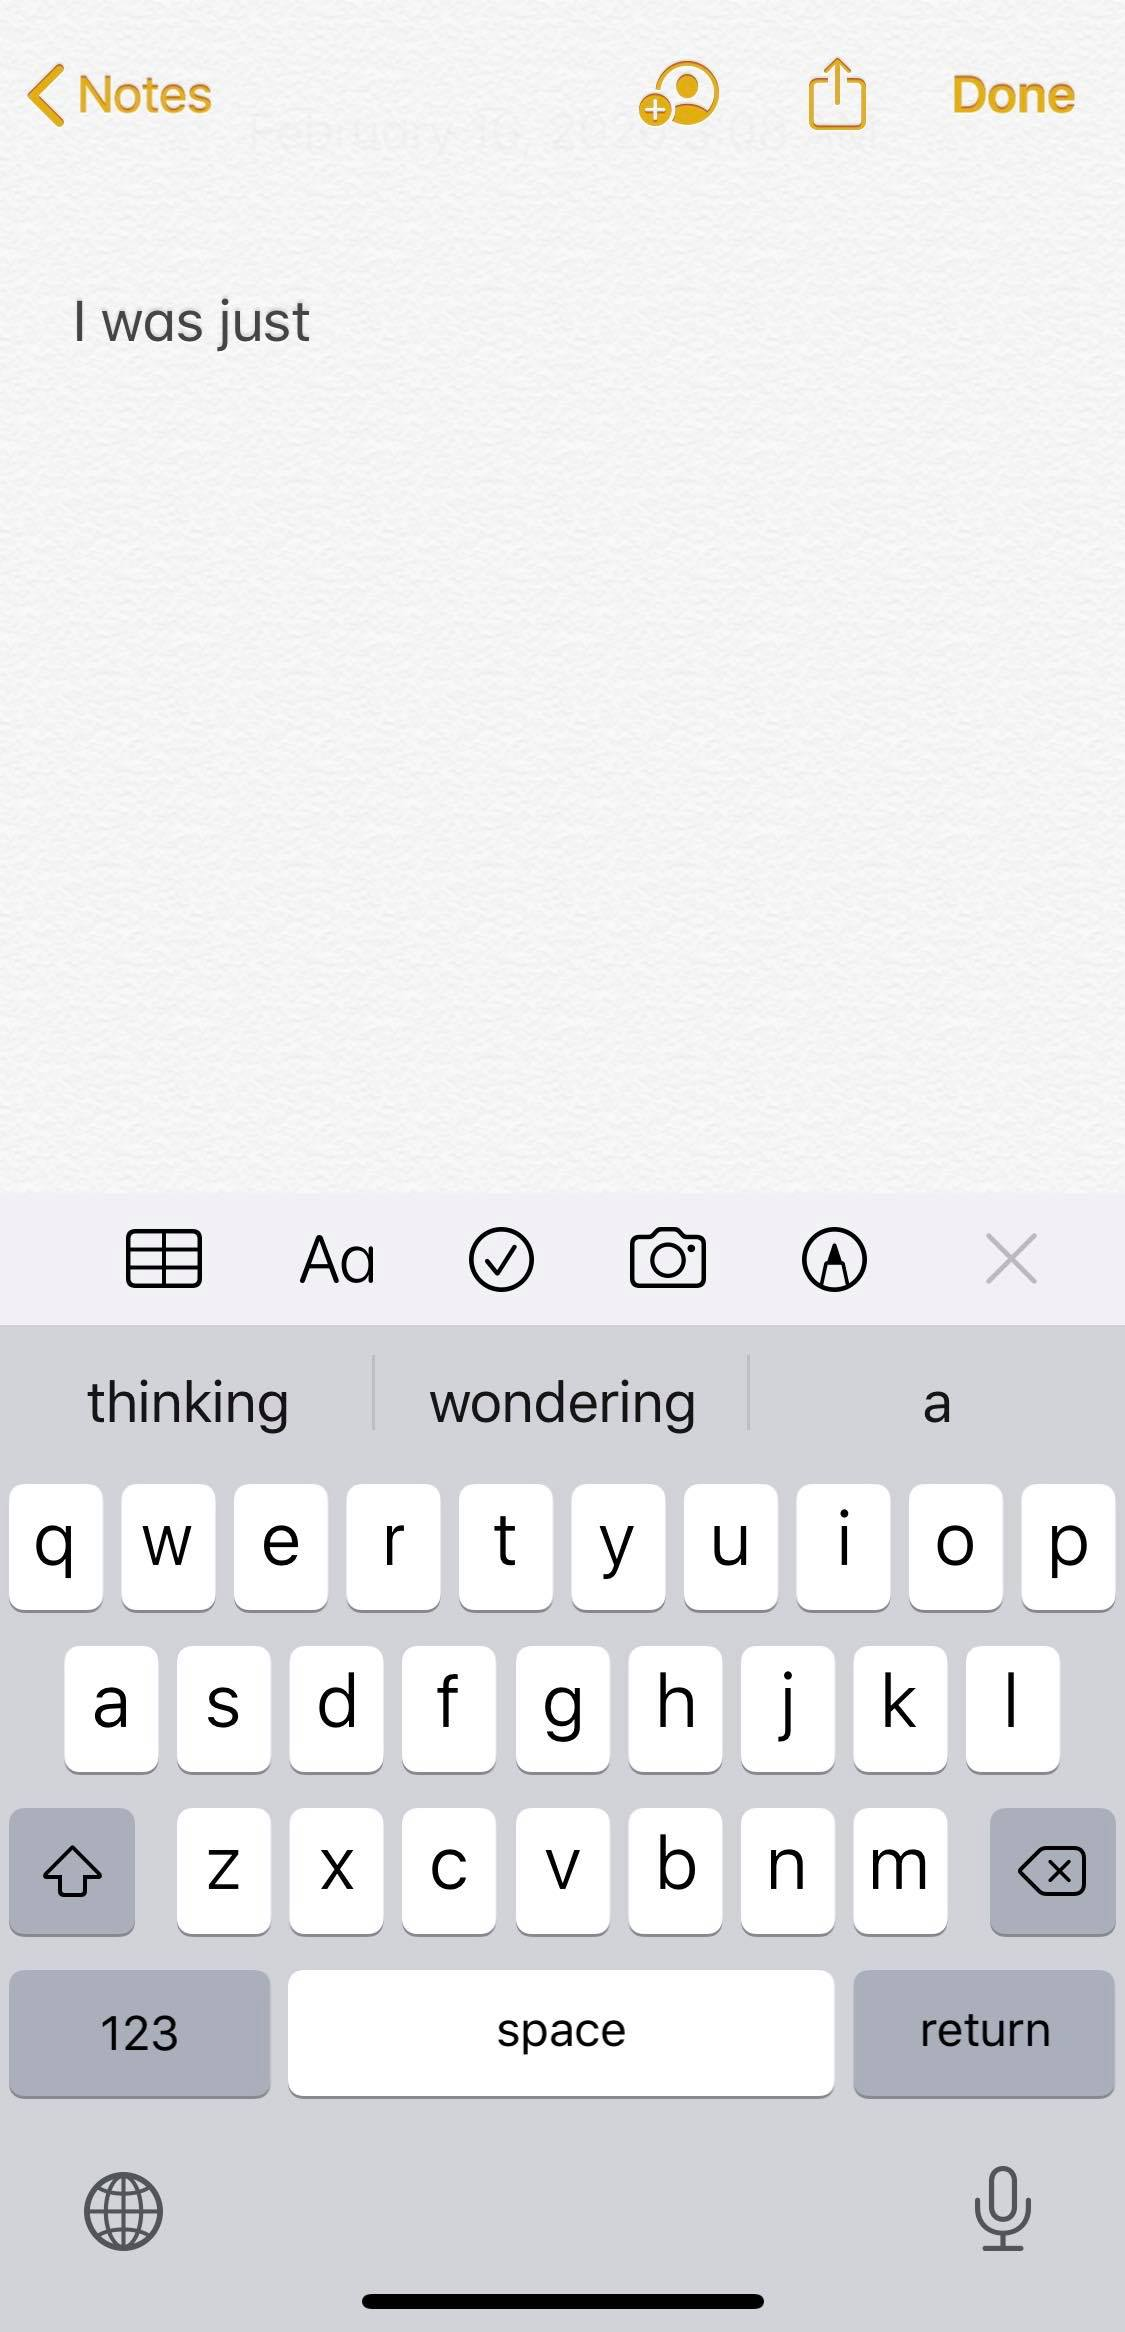
\includegraphics[width=3cm]{third}}
\end{frame}

%%%%%%%%%%%%%%%%%%%%%%%%%%%%%%%%%%%%%%%%%%%%%%%%%%%%%%%%%%%%%%%
\begin{frame}{How to \textcolor[rgb]{0.8,0.2,0}{Predict}?}
    \centering

    "I am japanese, so I speak" \visible<2->{$\rightarrow$} \visible<3->{"japanese"}
\end{frame}
%%%%%%%%%%%%%%%%%%%%%%%%%%%%%%%%%%%%%%%%%%%%%%%%%%%%%%%%%%%%%%%
\section{POS-Ngram}
\subsection{Definitions}

\begin{frame}{What does POS-Ngram mean?}
    \begin{definition}{Part of Speech (POS)}
        one of the classes into which words are divided according to their grammar,
        such as noun, verb, adjective, etc.
    \end{definition}
    \begin{definition}{N-gram}
        is a contiguous sequence of n items from a given sample of text or speech
        \begin{itemize}
            \item \textbf{unigram (1-gram)} : (I,), (study,), (english,)
            \item \textbf{bigram (2-gram)} : (I, study), (study, english) 
            \item \textbf{trigram (3-gram)} : (I, study, english)
        \end{itemize}
    \end{definition}
\end{frame}

%%%%%%%%%%%%%%%%%%%%%%%%%%%%%%%%%%%%%%%%%%%%%%%%%%%%%%%%%%%%%%%
\begin{frame}{What does POS-Ngram mean?}
    \begin{definition}{N-gram model}
        is one of statistical langauge models for predicting the next item (word) based on Markov assumption, and usually abbreviated as N-gram.
    \end{definition}
    \begin{definition}{POS-Ngram}
        is an improved model using part of speech as a class indicator.
    \end{definition}
\end{frame}

%%%%%%%%%%%%%%%%%%%%%%%%%%%%%%%%%%%%%%%%%%%%%%%%%%%%%%%%%%%%%%%
\subsection{N-gram}

\begin{frame}{How To Compute Probability of a Sentence?}
How can we compute the joint probability of a sentence?\\
\textit{Ex:} "an apple is on the" \\
    $$P(an\ apple\ is\ on\ the) = \text{?}$$

\end{frame}
%%%%%%%%%%%%%%%%%%%%%%%%%%%%%%%%%%%%%%%%%%%%%%%%%%%%%%%%%%%%%%%
\begin{frame}{Chain Rule Of Probability}
    \begin{block}{\textcolor[rgb]{0.8,0.2,0}{Notation}}
        \visible<1->{\begin{itemize}
            \visible<2->{\item To represent the probability of a paricular random variable $X_i$ taking on the value "the", or $P(X_i="the")$ we will use simplification $P(the)$.}
            \visible<3->{\item We represent a sequence of N words either as $w_1\cdots w_n$ or $w_1^n$}
        \end{itemize}}
    \end{block}

\end{frame}
%%%%%%%%%%%%%%%%%%%%%%%%%%%%%%%%%%%%%%%%%%%%%%%%%%%%%%%%%%%%%%%

\begin{frame}{Chain Rule Of Probability}
    \visible<1->{\begin{block}{In General}
        $$P(X_1\cdots X_n) = P(X_1)P(X_2\mid X_1)P(X_3\mid X_1^2)\cdots P(X_n\mid X_1^{n-1})$$
    \end{block}}

    \visible<2->{\begin{block}{By applying chain rule to a sequence of words}
        $$P(w_1\cdots w_n) = P(w_1)P(w_2\mid w_1)P(w_3\mid w_1^2)\cdots P(w_n\mid w_1^{n-1})$$
    \end{block}}

    \visible<3->{\begin{block}{Examples}
        \begin{itemize}
            \item $P(an\ apple) = P(an)\times P(apple\mid an)$
            \item $P(an\ apple\ is) = P(an)\times P(apple\mid an) \times P(is\mid an\ apple)$
        \end{itemize}
    \end{block}}

\end{frame}
%%%%%%%%%%%%%%%%%%%%%%%%%%%%%%%%%%%%%%%%%%%%%%%%%%%%%%%%%%%%%%%

\begin{frame}{Let's Apply Chain Rule}
By applying chain rule to the phrase $"an\ apple\ is\ on\ the"$:
    \begin{align*}
        P("an\ apple\ is\ on\ the") &= P(an)\times P(apple|an) \times P(is|an\ apple)\\
                                  &\times P(on|an\ apple\ is) \times P(the|an\ apple\ is\ on) 
    \end{align*}
\end{frame}
%%%%%%%%%%%%%%%%%%%%%%%%%%%%%%%%%%%%%%%%%%%%%%%%%%%%%%%%%%%%%%%

\begin{frame}{In practice chain rule does not help}
    \begin{itemize}
        \item We don't know the way to compute the exact probability of a word given a long sequence of preceding words, $P(w_n|w_n^{n-1})$
        \item Language is creative, and any particular context might have never occured before
    \end{itemize}
    \begin{block}{Example}
        $$P(sentences\mid this\ is\ an\ example\ of\ long) = \mathord{?}$$
    \end{block}
\end{frame}
%%%%%%%%%%%%%%%%%%%%%%%%%%%%%%%%%%%%%%%%%%%%%%%%%%%%%%%%%%%%%%%

\begin{frame}{The Presence of N-gram}
    The general equation for this n-gram approximation to the conditional probability of the next word in a sequence is
    $$P(w_n|w_1^{n-1}) \approx P(w_n|w_{n-N+1}^{n-1})$$

    \visible<2->{\begin{block}{In case of Bigram (2-gram)}
        When we use bigram model to predict the conditional probability of the next word, we can approximate by
        $$P(w_n|w_1^{n-1}) \approx P(w_n|w_{n-1})$$
    \end{block}}

    \visible<3->{\begin{block}{Example}
        $$P(the|\ an\ apple\ is\ on) \approx P(the|\ on)$$
    \end{block}}
\end{frame}

%%%%%%%%%%%%%%%%%%%%%%%%%%%%%%%%%%%%%%%%%%%%%%%%%%%%%%%%%%%%%%%

\begin{frame}{Bigram in Practice}
By supposing that C is the counts of word from a corpus.
    $$P(w_n|w_{n-1}) = \frac{C(w_{n-1}w_n)}{\sum_{w}C(w_{n-1}w)}$$

    \visible<2->{\begin{block}{Example}
        $$P(the|\ on) = \frac{C(on\ the)}{\sum_{others}C(on\ others)}$$
    \end{block}}
\end{frame}

%%%%%%%%%%%%%%%%%%%%%%%%%%%%%%%%%%%%%%%%%%%%%%%%%%%%%%%%%%%%%%%

\begin{frame}{The probability of a complete word sequence}
    Given the \textbf{bigram} assumption for the probability of an individual word, we can compute the probability of complete word sequence by:
    $$P(w_1^n) \approx \prod_{k=1}^nP(w_k\mid w_{k-1})$$

    \visible<2->{\begin{block}{Example}
        \begin{align*}
            P(an\ apple\ is\ on\ the) &= P(apple\mid an) \times P(is\mid apple) \times P(on\mid is)\\
                                      &\times P(on\mid is) \times P(the\mid on)
        \end{align*}
    \end{block}}

\end{frame}

%%%%%%%%%%%%%%%%%%%%%%%%%%%%%%%%%%%%%%%%%%%%%%%%%%%%%%%%%%%%%%%

\begin{frame}{OOV \& Smoothing}
    \textbf{OOV} stands for \textbf{Out Of Vocabulary}\\
    \begin{itemize}
        \item Words appear only in a test set but not in the training set.
        \item OOV problem occurs even when we work on big data.
    \end{itemize}
\end{frame}
%%%%%%%%%%%%%%%%%%%%%%%%%%%%%%%%%%%%%%%%%%%%%%%%%%%%%%%%%%%%%%%

\begin{frame}{Types of smoothing}
    \begin{itemize}
        \item Laplace smoothing (Add-one smoothing)
        \item Add-k smoothing
        \item Interpolation
        \item $\cdots$
    \end{itemize}
    \begin{block}{Interpolation}
        We mix the probability estimates from all the n-gram estimators, weighing and combining the trigram, bigram, and unigram counts.
    \end{block}
\end{frame}
%%%%%%%%%%%%%%%%%%%%%%%%%%%%%%%%%%%%%%%%%%%%%%%%%%%%%%%%%%%%%%%

\begin{frame}{Interpolation}
    To estimate $P(w_n\mid w_{n-2}w_{n-1})$ we use simple interpolation as follows:

    \visible<2->{\begin{block}{In case of Bigram}
        $$\hat{P}(w_n\mid w_{n-1}) = \lambda_1P(w_n\mid w_{n-1}) + \lambda_2P(w_n)$$
    \end{block}}

    \visible<3->{\begin{block}{In case of Trigram}
        \begin{align*}
            \hat{P} (w_n|w_{n-2}w_{n-1}) &= \lambda_1P(w_n|w_{n-2}w_{n-1})\\
                                         &+ \lambda_2P(w_n|w_{n-1})\\
                                         &+ \lambda_3P(w_n)
        \end{align*}
    \end{block}}

    \visible<4->{where we choose $\lambda_i$ such that $\sum_i\lambda_i = 1$}
\end{frame}
%%%%%%%%%%%%%%%%%%%%%%%%%%%%%%%%%%%%%%%%%%%%%%%%%%%%%%%%%%%%%%%

\begin{frame}{How are the $\lambda$ values set?}
    \begin{itemize}
        \item They can be learned from a \textbf{held-out} corpus
        \item Can be found by \textbf{EM} algorithm
        \item For the purpose of this project, we assume without loss of generality that $\lambda_i > \lambda_j (\forall i < j)$
    \end{itemize}
\end{frame}
%%%%%%%%%%%%%%%%%%%%%%%%%%%%%%%%%%%%%%%%%%%%%%%%%%%%%%%%%%%%%%%

\subsection{POS-Ngram}
\begin{frame}{POS-Ngram}

    \begin{block}{Formula}
        $$P(w_n\mid w_1^{n-1}) = \sum_{c_n}P(w_n\mid c_n)\times P(c_n\mid c_{n-N+1}^{n-1})$$
    \end{block}

    \visible<2->{\begin{block}{Example}
        \centering
        \begin{tabular}{|l|l|}
            \hline
            $c_1$:Noun & cat, dog, thought, $\cdots$\\\hline
            $c_2$:Verb & go, speak, $\cdots$\\\hline
            $c_1$:Noun, $c_2$:Verb & play, $\cdots$\\\hline
        \end{tabular}\\
    \end{block}}

    \flushleft
    
    \visible<3->{It means that to predict the next word $w_n$
    \begin{enumerate}
        \item Compute $P(c_n|c_{n-N+1}^{n-1}) \sim P(w_n|w_{n-N+1}^{n-1})$ 
        \item $P(w_n\mid c_n)=\frac{C(w_n,c_n)}{C(c_n)}$
        \item $w_n^\ast$ is defined by $\argmax_{w_n} P(w_n\mid w_1^{n-1})$
    \end{enumerate}}
\end{frame}
%%%%%%%%%%%%%%%%%%%%%%%%%%%%%%%%%%%%%%%%%%%%%%%%%%%%%%%%%%%%%%%
\section{Implementation}
%%%%%%%%%%%%%%%%%%%%%%%%%%%%%%%%%%%%%%%%%%%%%%%%%%%%%%%%%%%%%%%
\subsection{Programming Structure}
\begin{frame}{Programming Structure}
    \smartdiagramset{}
    \begin{center}
        \smartdiagram[priority descriptive diagram]{PosNgram.py,Predict.py,Ui.py}
    \end{center}
\end{frame}
%%%%%%%%%%%%%%%%%%%%%%%%%%%%%%%%%%%%%%%%%%%%%%%%%%%%%%%%%%%%%%%

\subsection{Tools}
\begin{frame}{Implementation}
    \begin{itemize}
        \item Programming Language : Python
        \item Ui : Tkinter
        \item NLTK (Natural Language ToolKit)
    \end{itemize}
    \begin{table}
        \flushleft
        \begin{tabular}{|l|l|l|}
            \hline
            \textbf{Function} & \textbf{Argument} & \textbf{Result}\\\hline
            word\_tokenize & "I like english." & ["I", "like", "english", "."]\\\hline
            pos\_tag & ["I", "like"] & [("I", "PRN"), ("like", "VBP")]\\
            \hline
        \end{tabular}
    \end{table}
\end{frame}

%%%%%%%%%%%%%%%%%%%%%%%%%%%%%%%%%%%%%%%%%%%%%%%%%%%%%%%%%%%%%%%

\begin{frame}{References}
    \begin{enumerate}
        \item Speech and Language Processing (Chapter 4) (Daniel Jurafsky - Stanford University, 1999)
        \item N-gram Language Modeling Tutorial (Lecture notes courtesy of Prof. Mari Ostendorf, 2007-06-21)
        \item Probabilistic Language Model (Chapter 3) (Kenji KITA, University of Tokyo Press, 1999)
    \end{enumerate}
\end{frame}
%%%%%%%%%%%%%%%%%%%%%%%%%%%%%%%%%%%%%%%%%%%%%%%%%%%%%%%%%%%%%%%

\begin{frame}
    \centering
    \Huge DEMO
\end{frame}

%%%%%%%%%%%%%%%%%%%%%%%%%%%%%%%%%%%%%%%%%%%%%%%%%%%%%%%%%%%%%%%

\begin{frame}
    \centering
    \Huge Thank You.
\end{frame}

%%%%%%%%%%%%%%%%%%%%%%%%%%%%%%%%%%%%%%%%%%%%%%%%%%%%%%%%%%%%%%%
\end{document}
